\documentclass[10pt]{article}
% Puedes usar esto (u otra codificaci\'on) si quieres:
\usepackage{graphicx}
\usepackage[utf8]{inputenc} %para usar acentos por ejemplo
\usepackage[spanish]{babel}  % para que las directivas del latex se impriman en españos. Por ejemplo \begin{abstract} ... \end{abstract}, aparecería "Abstract", pero con este paquete aparecerá "Resumen"
\usepackage{imakeidx}
\usepackage{listings}
\usepackage{float}
\usepackage{hyperref}

\makeindex[columns=3]

\title{Metaheurísticas Poblacionales} % El titulo debería ser lo mas descriptivo y conciso posible
\author{Rosas Francisco, Gurruchaga Luciano}

\date{\today} % Eliminar \today y no pone la fecha actual según se indica: \date{}

\begin{document}

% Agrega el título
\maketitle

\begin{abstract}

El objetivo de este documento será el estudio, análisis y comparación de dos Metaheurísticas Poblacionales, los Algoritmos Genéticos \textbf{GA} y la Evolución Diferencial \textbf{DE}. Los mismos serán sometidos a una serie de pruebas con funciones, las funciones de testeo \textit{Ackley 1, Ackley 2, Ackley 3 y Ackley 4 }. Luego, se verá el desempeño de dichos algoritmos descubriendo cuál es el método más adecuado para la resolución de problemas en un espacio grande de soluciones complejas de optimizar.

Se comenzará con la definición de conceptos básicos necesarios, el estado actual de las metaheurísticas poblacionales, y expondremos las  implementaciones y consideraciones de las soluciones. Finalmente, se procederá a la comparación de los resultados del objeto de estudio.

\end{abstract}

%----------------------------------------------------------------------------------------
%	Contenido del artículo
%----------------------------------------------------------------------------------------

\section{Introducción}

Una metaheurística del griego "meta" ("más allá") y "heurístico" ("encontrar") es un proceso o método heurístico de alto nivel diseñado para resolver un tipo de problema de optimización, usando parámetros dados por el usuario sobre unos procedimientos genéricos y abstractos buscando obtener la mejor solución o al menos, una solución aproximada eficiente, especialmente con información incompleta o imperfecta, o capacidad de cómputo limitada.

Las metaheurísticas son aplicadas cuando un problema dado no cuenta con un algoritmo o heurística especifica que de una solución satisfactoria al problema o, la implementación de dicho algoritmo no es posible, ya sea por tiempo, espacio o simplemente la tecnología actual no está a la altura.

Las metaheurísticas pueden hacer relativamente pocas suposiciones sobre el problema de optimización que se está resolviendo y, por lo tanto, pueden usarse para una variedad de problemas

\subsection*{Clasificacion de Metaheuristicas}
Existen distintas maneras de clasificar una metaheurística, nos enfocaremos en dos tipos: Metaheurísticas inspiradas en la Naturaleza y Metaheurísticas Poblacionales.

El enfoque poblacional mantiene y mejora múltiples soluciones candidatas, a menudo utilizando características de la población para guiar la búsqueda, a diferencia de enfoques de solución única, los cuales se centran en modificar y mejorar una única solución candidata.

El diseño de metaheuristicas inspiradas en la naturaleza, especialmente los algoritmos basados en computación evolutiva, están fuertemente inspiradas en sistemas naturales como pueden ser la organización de ciertas especies (lobos, hormigas, abejas, etc.), sistemas más "generales" como las leyes de la física o naturaleza (gravedad, selección natural, etc.). 

La naturaleza actúa como una fuente de conceptos, mecanismos y principios para el diseño de sistemas informáticos artificiales para hacer frente a problemas informáticos complejos.

\subsection{\textbf{GA}- Algoritmo Genético }

Un algoritmo genético es una metaheurística poblacional inspirada en el proceso de la selección natural.

Se trabaja con un conjunto de soluciones al que llamaremos \textbf{población}, cada solución particular o \textbf{individuo} es representada por medio de un vector de valores discretos llamado \textbf{cromosomas}. A los símbolos que conforman dichos vectores se les llama \textbf{genes}. Los cromosomas evolucionan a lo largo de distintas iteraciones, las llamadas \textbf{generaciones}. En cada generación, los cromosomas son evaluados usando alguna medida de aptitud o función objetivo. Las siguientes generaciones, nuevos cromosomas, son generadas aplicando operadores genéticos repetidamente a la generación actual, siendo estos los operadores de selección (selection), cruzamiento (crossover), mutación (mutation) y reemplazo.

\subsection{\textbf{DE}- Evolución Diferencial }
En la computación evolutiva (Familia de algoritmos de optimización global inspirados en la evolución biológica - rama de la Inteligencia Artificial)[2], evolución diferencial es un método que optimiza un problema intentando mejorar una solución candidata iterativamente con respecto a una medida de calidad determinada. Estos métodos son comúnmente conocidos como "Metaheurísticas", ya que no hace ninguna suposición(o muy pocas) sobre el problema que se está optimizando y puede buscar espacios muy grandes de soluciones candidatas. Sin embargo, las metaheurísticas como DE no garantizan encontrar la solución óptima.

DE es usado para funciones multidimensionales de valores Reales, sin utilizar el "gradiente" del problema a ser optimizado, en otras palabras, DE no requiere o no necesita que el problema a optimizar sea diferenciable, como en el clásico caso del método de "descenso del gradiente" [3] o "Quasi-Newton method" [4]. Por lo tanto, la evolución diferencial también puede utilizarse en problemas de optimización que ni siquiera son continuos, son ruidosos, cambian con el tiempo, etc.

La DE optimiza un problema manteniendo una población de soluciones candidatas y creando nuevas soluciones candidatas, combinando las existentes según sus sencillas fórmulas, y quedándose con la solución candidata que tenga la mejor puntuación o aptitud en el problema de optimización en cuestión. De este modo, el problema de optimización se trata como una caja negra que simplemente proporciona una medida de calidad dada una solución candidata y, por tanto, el gradiente no es necesario.

La DE fue introducida por Storn y Price en la década de 1990. Se han publicado libros sobre los aspectos teóricos y prácticos del uso de la ED en la computación paralela, la optimización multiobjetivo y la optimización restringida, y muchos otros estudios en diversas áreas de aplicación. 

\subsection{Funciones Akcley}

Las funciones de prueba son una excelente herramienta para validar y comparar el rendimiento de distintos algoritmos de optimización

Si bien se han publicado muchas funciones de prueba o de referencia, no existe una lista o conjunto estándar de funciones. Lo ideal es que las funciones de prueba deben tener diversas propiedades para que puedan ser realmente útiles para probar nuevos algoritmos de una de forma imparcial.

En general, los problemas sin restricciones pueden clasificarse en dos categorías: funciones de prueba y los problemas del mundo real.

Las funciones de prueba son problemas artificiales, y pueden utilizarse para evaluar el comportamiento de un algoritmo en situaciones a veces diversas y difíciles. Los problemas artificiales pueden incluir un único mínimo global, uno o varios mínimos globales en presencia de muchos mínimos locales, valles largos y estrechos, efectos de espacio nulo y superficies planas. 

Por otro lado, los problemas del mundo real se originan en diferentes campos como la física, la química ingeniería, matemáticas, etc. Estos problemas son difíciles de manipular y pueden contener expresiones algebraicas o diferenciales complicadas y pueden requerir una cantidad significativa de datos para compilarlos.

Una función con más de un óptimo local se denomina multimodal. Estas funciones se utilizan para probar la capacidad de un algoritmo para escapar de cualquier mínimo local. Si el proceso de exploración de un algoritmo está mal diseñado, entonces no puede buscar en el paisaje de funciones de manera efectiva. Esto, a su vez, hace que un algoritmo se quede atascado en un mínimo local. Las funciones multimodales con muchos mínimos locales se encuentran entre la clase de problemas más difícil para muchos algoritmos. 

Las funciones con superficies planas suponen una dificultad para los algoritmos, ya que la planitud de la función no da al algoritmo ninguna información para dirigir el proceso de búsqueda hacia los mínimos.

Una función de p variables se llama separable, si se puede escribir como una suma de p funciones de una sola variable

Entonces, la comprobación del comportamiento, la fiabilidad, la eficiencia y la validación de los algoritmos de optimización se lleva a cabo con frecuencia utilizando un conjunto elegido de puntos de referencia estándar comunes o funciones de prueba de la literatura.[5]

\section{Descripción del Problema}

En este breve trabajo de estudio de metaheurísticas poblacionales, utilizaremos los dos enfoques o modelos algorítmicos descritos en la sección previa. GA y DE, los cuales implementaremos y pondremos a prueba frente a un conjunto acotado de funciones de prueba extraídas de la bibliografía[5], para, luego de extraer los resultados obtenidos, realizar un análisis comparativo de su comportamiento frente a diversos aspectos.


\subsection{Conjunto de funciones Ackley a utilizar}
%$  X  $

\textbf{Ackley 1 Function: } (continua, diferenciable, no separable, escalable, multimodal)
 $$ f_1(x) = -20e^{-0.02}\sqrt{D^{-1}\sum_{i=1}^{D}x_{i}^2}-e^{D-1\sum_{i=1}^{D}cos(2\pi x_i)}+20+e$$
\textbf{Óptimo global del intervalo} 
$$[-35\leq x_i \leq 35], x^* = (0,..., 0), f_1(x^*) = 0$$

\textbf{Akcley 2  Function:  } (continua, diferenciable, no separable, no escalable,unimodal)
$$ f_2(x) = -200e^{-0.02}\sqrt{x_1^2+x_2^2}$$
\textbf{Óptimo global del intervalo}
 $$[-32\leq x_i \leq 32], x^* = (0,0), f_2(x^*) = -200$$

\textbf{Akcley 3  Function:  } (continua, diferenciable, no separable, no escalable, unimodal)
$$ f_3(x) = 200e^{-0.02}\sqrt{x_1^2+x_2^2}+5e^{cos(3x_1)+sin(3x_2)}$$
\textbf{Óptimo global del intervalo} 
$$[-32\leq x_i \leq 32], x^* = (0, \approx -0.4), f_3(x^*) \approx -219.1418$$

\textbf{Akcley 4  Function: } (continua, diferenciable, no separable, escalable, multimodal)
$$f_4(x) =  \sum_{i=1}^{D}(e^{-0.2}\sqrt{x_i^2+x_{i+1}^2}+3(cos(2x_i)+sin(2x_{i+1}))$$
\textbf{Óptimo global del intervalo} 
$$[-35\leq x_i \leq 35], x=f(\{-1.479252,-0.739807\},\{1.479252,-0.739807\}), f(x^*) \approx -3.917275$$ 

\section{Propuesta algorítmica} % El titulo de esta y el resto de las secciones es orientativa

\subsection{El algoritmo Genetico}

Contamos con una población $P$, dicha población está formada por un conjunto de soluciones individuos $I$, cada individuo $I$ está representado por un conjunto de cromosomas, los cuales a su vez están formados una secuencia de genes $g_i$ de valor discreto, que representan una solución al problema, formalmente:

$$P =\{i_0,i_1,..,i_n\}$$
$$I =\{(g_0,g_1,..,g_n)_0,(g_0,g_1,..,g_n)_1,...,(g_0,g_1,..,g_n)_n\}$$

Se toman todos los individuos de la población $I \in P$, se obtiene una medida de "desempeño" (las funciones Ackley seran nuestra medida de desempeño) de cada solución $I$, aquellos con mejor desempeño son más propensos a reproducirse, como sucede en la selección natural, donde los más aptos sobreviven y tienen más posibilidades de trasmitir sus genes.

Existen distintas formas de seleccionar que individuos se reproducen, nosotros utilizaremos la \textit{"selección basada en torneos"} la cual consiste en seleccionar de forma aleatoria dos individuos distintos de la población, y, aquel con mejor desempeño será quien pueda reproducirse y, por tanto, sus genes serán "heredados" en la siguiente población $P$. Sumado a esto, existe una probabilidad de cruza y mutación de los genes al reproducirse.

Para la primera utilizaremos el operador de cruce \textbf{PMX} o \textit{cruce por emparejamiento parcial}. Consiste en elegir un sub-segmento de los genes de uno de los progenitores y cruzarlos, preservando el orden y la posición de la mayor cantidad de genes posible del otro manteniendo la coherencia.
En cuanto a la mutación, tomaremos un gen aleatorio y (basado en una probabilidad) le sumaremos o restaremos un escalar proporcional a la distancia del valor del gen a los límites permitidos.

A medida que avanzan las generaciones, en cada población irán quedando aquellos individuos que cuentan con los "mejores" genes de generaciones anteriores, por tanto, los de mejor desempeño. Recuperando al mejor individuo histórico (de todas las generaciones) obtenemos una solución aproximada aceptable.

\subsection{El algoritmo Evolucion Diferencial}

La evolución diferencial es un enfoque heurístico para la optimización global de funciones espaciales continuas, no lineales y no diferenciables. 

El algoritmo comienza iniciando aleatoriamente una población de vectores de decisión de valor real, también conocidos como genomas o cromosomas. Estos representan las soluciones candidatas al problema de optimización multidimensional.\newline
En cada iteración, el algoritmo introduce mutaciones en la población para generar nuevas soluciones candidatas. El proceso de mutación añade la diferencia ponderada entre dos vectores de la población a un tercer vector, para producir un vector mutado. Los parámetros del vector mutado se mezclan de nuevo con los parámetros de otro vector predeterminado, el vector objetivo, durante un proceso conocido como cruce que pretende aumentar la diversidad de los vectores de parámetros perturbados. El vector resultante se conoce como vector de prueba.
Estas mutaciones se generan de acuerdo con una estrategia de mutación, que sigue una convención de nomenclatura general de $DE/x/y/z$ , donde DE significa Evolución Diferencial, mientras que x denota el vector a ser mutado, y denota el número de vectores de diferencia considerados para la mutación de x, y z es el tipo de cruce en uso. Por ejemplo, las estrategias populares

$ DE/rand/1/bin y DE/best/2/bin $ especifican que el vector x puede elegirse al azar (rand) de la población, o bien se selecciona el vector con el menor coste (best); que el número de vectores de diferencia considerados es 1 o 2; y que el cruce se realiza según experimentos binomiales independientes (bin).

Una última operación de selección sustituye el vector objetivo, o el padre, por el vector de prueba, su descendiente, si este último arroja un valor de función objetivo menor. De este modo, el descendiente más apto se convierte en un miembro de la nueva población generada, y posteriormente participa en la mutación de otros miembros de la población. Estas iteraciones continúan hasta que se alcanza un criterio de terminación. (como el agotamiento de las evaluaciones funcionales máximas).

El algoritmo de evolución diferencial requiere muy pocos parámetros para funcionar, a saber, el tamaño de la población, NP, un factor de escala real y constante, $F \in [0, 2] $, que pondera la variación diferencial durante el proceso de mutación, y una tasa de cruce, $ CR \in  [0, 1]$, que se determina experimentalmente. Esto hace que el algoritmo sea fácil y práctico de utilizar. [6]

En este caso utilizaremos un algoritmo de evolución diferencial con el esquema $ " DE/rand/1/bin " $ para ejecutar con las funciones Ackley.

\section{Resultados}%
A continuación mostraremos la evolución de las soluciones para cada Ackley en ambos algoritmos y las estadísticas de las mejores soluciones para cada función Ackley de cada algoritmo en veinte ejecuciones con diferentes semillas.

\begin{figure}[H]
\centerline{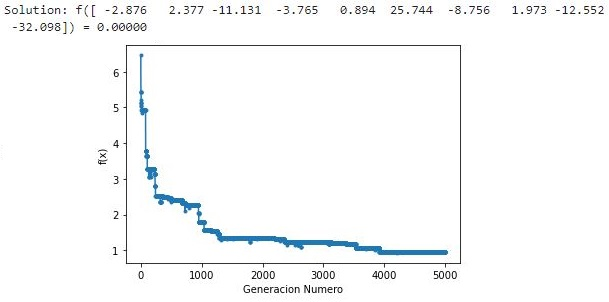
\includegraphics{ack-1-ga.jpg}}
\caption{Evolucion de la solución GA - Ackley1}
\label{fig_1}
\end{figure}

\begin{figure}[H]
\centerline{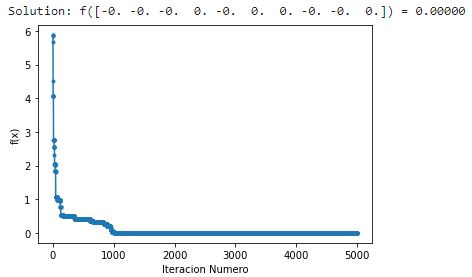
\includegraphics{ack-1-de.jpg}}
\caption{Evolucion de la solución DE - Ackley1}
\label{fig_2}
\end{figure}

\begin{figure}[H]
\centerline{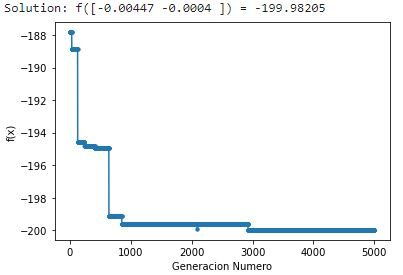
\includegraphics{ack-2-ga.jpg}}
\caption{Evolucion de la solución GA - Ackley2}
\label{fig_3}
\end{figure}

\begin{figure}[H]
\centerline{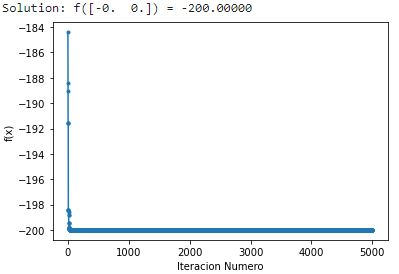
\includegraphics{ack-2-de.jpg}}
\caption{Evolucion de la solución DE - Ackley2}
\label{fig_4}
\end{figure}

\begin{figure}[H]
\centerline{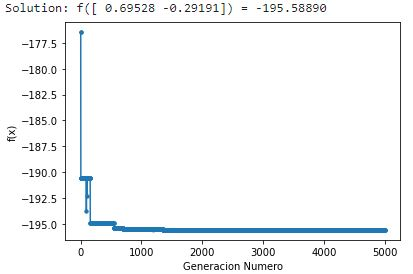
\includegraphics{ack-3-ga.jpg}}
\caption{Evolucion de la solución GA - Ackley3}
\label{fig_5}
\end{figure}

\begin{figure}[H]
\centerline{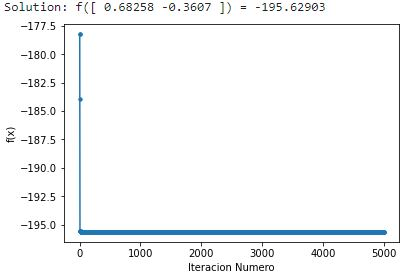
\includegraphics{ack-3-de.jpg}}
\caption{Evolucion de la solución DE - Ackley3}
\label{fig_6}
\end{figure}

\begin{figure}[H]
\centerline{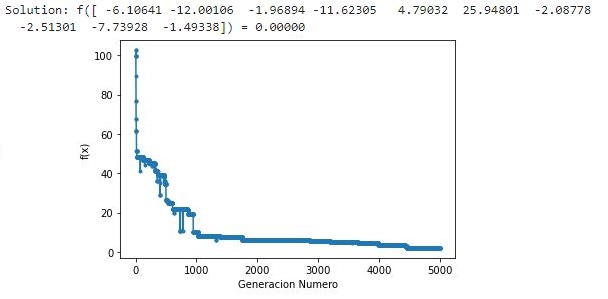
\includegraphics{ack-4-ga.jpg}}
\caption{Evolucion de la solución GA - Ackley4}
\label{fig_7}
\end{figure}

\begin{figure}[H]
\centerline{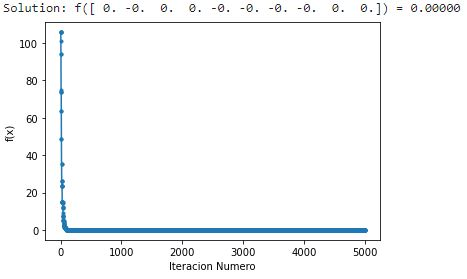
\includegraphics{ack-4-de.jpg}}
\caption{Evolucion de la solución DE - Ackley4}
\label{fig_8}
\end{figure}

Con solamente una ejecución podemos ver como DE encuentra la solución en muchas menos iteraciones que GA, además de encontrar la solución óptima global en Ackley 1, 2 y 3.

Al realizar veinticinco ejecuciones en veinticinco semillas diferentes obtuvimos las siguientes estadísticas de los mejores resultados por generación:

\subsection{Estadisticas Algoritmo Genetico}
GA-Ackley1
\begin{itemize}
\item
Media:  0.0 
\item%
Mediana:  0.0 
\item%
Desviacion:  0.0
\end{itemize}

GA-Ackley2
\begin{itemize}
\item
Media:  -199.79401210116922 
\item%
Mediana:  -199.78800235653605 
\item%
Desviacion:  0.13499328080135112
\end{itemize}

GA-Ackley3
\begin{itemize}
\item
Media:  -195.6091691677698 
\item%
Mediana:  -195.61744388914246 
\item%
Desviacion:  0.02448920551142561
\end{itemize}

GA-Ackley4
\begin{itemize}
\item
Media:  0.0 
\item%
Mediana:  0.0 
\item%
Desviacion:  0.0
\end{itemize}

\subsection{Estadisticas Evolucion Diferencial}

ED-Ackley 1
\begin{itemize}
\item
Media:  3.9968028886505635e-15 
\item%
Mediana:  3.9968028886505635e-15 
\item%
Desviacion:  0.0
\end{itemize}

ED-Ackley 2 
\begin{itemize}
\item
Media:  -200.0 
\item%
Mediana:  -200.0 
\item%
Desviacion:  0.0
\end{itemize}

ED-Ackley 3 
\begin{itemize}
\item
Media:  -195.62902826227938 
\item%
Mediana:  -195.62902826227938 
\item%
Desviacion:  0.0
\end{itemize}

ED-Ackley 4 
\begin{itemize}
\item
Media:  5.2969997997001116e-135 
\item%
Mediana:  0.0 
\item%
Desviacion:  2.5949893353779947e-134
\end{itemize}

\section{Conclusiones}
Como hemos visto, tanto GA y ED obtienen soluciones satisfactorias, pero, la diferencia es notable, ED se desempeña mejor en casi todos los aspectos, no solo obtiene la solución en muchas menos iteraciones, menos de 1500, sino que es capaz de encontrar el óptimo global en tres de cuatro funciones, a diferencia de GA que no pudo encontrar el óptimo global en ninguna.

Sin embargo, hay que considerar que si bien ED encontró una solución en menos iteraciones, las veinticinco ejecuciones con cinco mil generaciones tomo aproximadamente una hora y media, en contra parte, GA tomo menos de veinte minutos.


%------------------------------------------------ 
\section*{Agradecimientos}
Prof. Guillermo Leguizamon

%----------------------------------------------------------------------------------------
%	Listado de bibliografía consultada / Puede incluír sitios web
%----------------------------------------------------------------------------------------

\begin{thebibliography}{99} % Bibliography - this is intentionally simple in this template
\bibitem0.\t[Clinton Sheppard, 2018]{}Genetic Algorithms with Python
\bibitem1.\t[Wikipedia]{}\url{https://en.wikipedia.org/wiki/Genetic_algorithm}
\bibitem2.\t[Wikipedia]{}\url{https://en.wikipedia.org/wiki/Evolutionary_computation}
\bibitem3.\t[Wikipedia]{}\url{https://en.wikipedia.org/wiki/Gradient_descent}
\bibitem4.\t[Wikipedia]{}\url{https://en.wikipedia.org/wiki/Quasi-Newton_method}
\bibitem5.\t[Cornell University - Ithaca, New York]{}\url{https://arxiv.org/abs/1308.4008v1} A Literature Survey of Benchmark Functions For Global Optimization Problems
\bibitem6.\t[ Machine Learning Mastery ]{}\url{https://machinelearningmastery.com/differential-evolution-from-scratch-in-python } Differential Evolution from Scratch in Python


\end{thebibliography} 
\section*{Codigo compartido}
\begin{lstlisting}[language=Python]
def ackley_1(individuo):
    global D
    sum1 = 0.0
    sum2 = 0.0
    for g in individuo:
        sum1 = sum1 + g**2.0
        sum2 = sum2 + np.cos(2.0*np.pi*g)
    return -20.0*np.exp(-0.02*np.sqrt(sum1/D)) - np.exp(sum2/D) + 20 + np.e


def ackley_2(individuo):
    return -200*np.exp(-0.02*np.sqrt(individuo[0]**2+individuo[1]**2))

def ackley_3(individuo):
    return ackley_2(individuo)+5*np.exp(np.cos(3*individuo[0])+np.sin(3*individuo[1]))

def ackley_4(individuo):
    global D
    suma = 0.0
    i=0
    while (i+1 < D):
        suma = suma + np.exp(-0.2)*np.sqrt(individuo[i]**2+individuo[i+1]**2)
        +3*(np.cos(2*individuo[i])+np.sin(2*individuo[i+1]))
        i = i + 1
    return suma

def init_populations(pop_size = PSIZE):
    global D
    pop_1 = []
    pop_2 = []
    pop_3 = []
    pop_4 = []
    for i in range(pop_size):
        pop_1.append([random.uniform(-35, 35) for i in range(D)])
        pop_2.append([random.uniform(-32, 32), random.uniform(-32, 32)])
        pop_3.append([random.uniform(-32, 32), random.uniform(-32, 32)])
        pop_4.append([random.uniform(-35, 35) for i in range(D)])
    return [np.array(pop_1),np.array(pop_2),np.array(pop_3),np.array(pop_4)]

def calculate_fitness(pop,ackley):
    switch = {
        1: ackley_1,
        2: ackley_2,
        3: ackley_3,
        4: ackley_4
    }
    scores = []
    for ind in pop:
        scores.append(switch.get(ackley)(ind))
    return scores
\end{lstlisting}

\section*{Código del Algoritmo DE}
\begin{lstlisting}[language=Python]
# define crossover operation
def crossover(mutated, target, dims, cr):
    # generate a uniform random value for every dimension
    p = random.rand(dims)
    # generate trial vector by binomial crossover
    trial = [mutated[i] if p[i] < cr else target[i] for i in range(dims)]
    return trial

# define mutation operation
def mutation(x, F):
    return x[0] + F * (x[1] - x[2])

# define boundary check operation
def check_bounds(mutated, ackley):
    if ackley == 2 or ackley == 3:
         mutated_bound = np.clip(mutated, -32, 32)
    else:
        #Va de i hasta D                       tomando li & ls
        mutated_bound = [np.clip(mutated[i], -35, 35) for i in range(D)]
    return mutated_bound

def differential_evolution(ackley,pop,scores,best_score,best_scores_progress,seed):
    random.seed(seed)
    np.random.seed(seed)
    mejor_puntaje = float('inf')
    mejor_solucion = []
    obj_iter = list()
    
    tam_ind = len(pop[0])
    # Init, find the best performing vector of initial population
    best_score=np.min(scores)
    best_scores_progress.append(best_score)
    
    for generation in range(MAXG):
        #new_population=[]
        if best_score < mejor_puntaje:
            mejor_puntaje = best_score
            mejor_solucion = pop[np.argmin(scores)][:]
        # iterate over all candidate solutions
        for i in range(int(PSIZE)):
            # choose three candidates, a, b and c, that are not the current one
            candidates = [candidate for candidate in range(PSIZE) if candidate != i]
            a, b, c = pop[random.choice(candidates, 3, replace=False)]
            # perform mutation
            mutated = mutation([a, b, c], F)
            # check that lower and upper bounds are retained after mutation
            mutated = check_bounds(mutated, ackley)
            # perform crossover binomial
            trial = crossover(mutated, pop[i], tam_ind, Cr)
           
            # compute objective function value for target vector
            pop_arr = []
            pop_arr.append(pop[i])
            obj_target = calculate_fitness(pop_arr,ackley) 
            # compute objective function value for trial vector
            pop_trial = []
            pop_trial.append(trial)
            obj_trial = calculate_fitness(pop_trial,ackley)
            
            # perform selection
            if obj_trial[0] < obj_target[0]:
                # replace the target vector with the trial vector
                pop[i] = trial
                # store the new objective function value
                scores[i] = obj_trial[0]
                
        # find the best performing vector at each iteration
        best_score = np.min(scores)    
        best_scores_progress.append(best_score)
    return [mejor_puntaje, mejor_solucion]

\end{lstlisting}

\section*{Código del Algoritmo GA}
\begin{lstlisting}[language=Python]

def select_individual_by_tournament(population, scores):
    population_size = len(scores)
    # Pick individuals for tournament
    fighter_1 = random.randint(0, population_size-1)
    fighter_2 = random.randint(0, population_size-1)
    while(fighter_1==fighter_2):
        fighter_2=random.randint(0,population_size-1)
    # Get fitness score for each
    fighter_1_fitness = scores[fighter_1]
    fighter_2_fitness = scores[fighter_2]
    # Identify undividual with highest fitness
    # Fighter 1 will win if score are equal
    if fighter_1_fitness <= fighter_2_fitness:
        winner = fighter_1
    else:
        winner = fighter_2
    # Return the chromsome of the winner
    return population[winner, :]

def crossover(parent_1,parent_2):
    chromosome_length = len(parent_1)
    child1 = parent_1[:]
    child2 = parent_2[:]
    if chromosome_length == 2:
        child1[1] = parent_2[1]
        child2[1] = parent_1[1]
    else:
        alfa = random.random()
        pivote = math.floor((chromosome_length-1)*alfa)
        while pivote==0 or pivote == chromosome_length-1: #Esto en teoria nunca pasa
            alfa = random.random()
            pivote = math.floor((chromosome_length-1)*alfa)
        child1[pivote:] = parent_2[pivote:]
        child2[pivote:] = parent_1[pivote:]
    return child1, child2

def mutation(ind):
    chromosome_length = len(ind)
    i=random.randint(0,chromosome_length-1)
    if chromosome_length == 2:
        b = [-32,32]
    else:
        b = [-35,35]
    if random.random() < 0.5:
        ind[i] = ind[i] + random.random()*(b[1]-ind[i])
    else:
        ind[i] = ind[i] - random.random()*(ind[i]-b[0])
    return ind

def ejecucion_ga(pop,ackley,scores,best_score,best_scores_progress,seed):
    random.seed(seed)
    np.random.seed(seed)
    mejor_puntaje = float('inf')
    mejor_solucion = []
    for generation in range(MAXG):
        new_population=[]
        if best_score < mejor_puntaje:
            mejor_puntaje = best_score
            mejor_solucion = pop[np.argmin(scores)][:]
        for i in range(int(PSIZE/2)):
            parent_1 = select_individual_by_tournament(pop, scores)
            parent_2 = select_individual_by_tournament(pop, scores)
            #Evolucion
            if np.random.random()<PC:
                child_1, child_2 = crossover(parent_1, parent_2)
            else:
                child_1=parent_1
                child_2=parent_2
            #Mutacion
            if np.random.random()<PM:
                mutation(child_1)
            if np.random.random()<PM:
                mutation(child_2)
            new_population.append(child_1)
            new_population.append(child_2)
        pop=np.array(new_population)
        scores=calculate_fitness(pop,ackley)
        best_score=np.min(scores)
        best_scores_progress.append(best_score)
    return [mejor_puntaje, mejor_solucion]
\end{lstlisting}
\newpage
\tableofcontents
\end{document}